% Author Name: José Areia 
% Author Contact: jose.apareia@gmail.com
% Version: 1.0.3 - 18/04/2025
% Public Repository: https://github.com/joseareia/nob-article

% Packages & Document Configurations
\documentclass[twocolumn]{NobArticle}
% \runninghead{MSSC DCA YMCA}
\footertext{\textit{Journal X} (2025) 12:684}

% Title
\title{Breif Introduction to MSSC Solving Using DCA, Math 515 66}

% Authors
\author{
    Ian Picklo\textsuperscript{1}}
% \begin{figure}
%     \centering
%     \includegraphics[width=1\linewidth]{alg1.png}
%     \caption{Enter Caption}
%     \label{fig:enter-label}
% \end{figure}

% Affiliations
\date{
    \textsuperscript{\textbf{1}}
    College of Engineering and Mines, The University of North Dakota \\
}

% Abstract
\renewcommand{\maketitlehookd}{%
% \begin{abstract}
%     \noindent 
%     DCA, MSSC, and me
%     \medskip

%     \small{\textbf{Index Terms:} Clustering Algorithms, Difference of Convex Functions.}
% \end{abstract}
}

\begin{document}

\small
\maketitle

% Introduction
\section{Introduction}
Mean sum of squares clustering  (MSSC) is one formulation of the clustering problem. The solution is able to group like data in so called cluster. These are useful in a variety of applications, from data science to machine learning. The difficulty is computing the solution to the MSSC formulation effectively and efficiently. 

The following report follows the implementation of a DC algorithm for solving MSSC problems. Specifically, it provides an introduction to clustering of data, K-means clustering, and implementing a DCA formulation from \cite{an_minimum_2009} to compare with. 

% Contribution
% \subsection{Contribution}
% This paper as the follow contributions.

% \begin{itemize}
% 	\item Arcu eros accumsan lorem, at posuere mi diam sit .
% 	\item Fusce fermentum, mi sit amet euismod rutrum.
% 	\item Sem lorem molestie diam, iaculis aliquet sapien tortor.
% 	\item Pellentesque bibendum pretium aliquet.
% \end{itemize}

% Paper Organisation
% \subsection{Paper Organisation}
% \blindtext

% \usepackage{amsthm}
% \theoremstyle{plain}
\newtheorem{lemma}{Lemma}
\newtheorem{sublemma}{Lemma}[lemma]
\newtheorem{theorem}{Theorem}[section]

\section{Background}
% \blindtext
This section is designed to give an the numerical tools for construction optimizations for MSSC. It will first cover on of the more traditional methods before giving an overview on how DC programming may be adapted as well. 
% \subsection{Literature Review}


\subsection{Mean Sum of Squares}
Square error algorithms, such as Mean Sum of Squares (MSSC), are some of the most frequently used classical methods for clustering data of distinct sets. These usually take the form of minimizing the distance between a set of n points/entities within a $c$ clusters to each cluster's centroid. For convenience, we will present using the notation present in \cite{an_minimum_2009}. Mathematically, this can be formulated as having $n$ entities be denoted as \(X := \{x_1, x_2, \ldots, x_n\} \in \mathbb{R}^d\). These are partitioned into \(c (2\le c\le n) \) clusters. The identification of which cluster element \(n\) is part of can be easily represented as \(U = (u_{i,k}) \in \mathbb{R}^{c\times n}\) with \(i =1,...,c\) and \(k =1,...,n.\) or as



    % Definition of the assignment variables
\[
u_{i,k} :=
\begin{cases}
1, & \text{if } x_k \in C_i,\\
0, & \text{otherwise}.
\end{cases}
\]
\noindent Further, with centriods $v_i \in \mathbb{R}^d$ and  the matrix \(V \in \mathbb{R}^{c\times d}\) where each column is $v_i$, MSSC can be formulated as 
% MSSC formulation
% \begin{equation}
\begin{equation}
\begin{cases}
\min{ f(U,V)}
:=  \sum_{k=1}^n \sum_{i=1}^c u_{i,k} \,\bigl\lVert x_k - v_i\bigr\rVert^2, \\[8pt]
\text{s.t.}\quad
u_{i,k} \in \{0,1\}, 
\quad i = 1,\dots,c,\; k = 1,\dots,n,\\[8pt]
\sum_{i=1}^c u_{i,k} = 1,\quad k = 1,\dots,n.
\end{cases}\\
\label{eq:my_equatio}
\end{equation}

\noindent These formulations can be uses with several optimization algorithms such as K-means and DCA.


\subsection{K-means}
%cover overview ith algorithm --baseline comparison 
One of the benchmark algorithms in clustering is the K-means algorithm introduced in \cite{macqueen_methods_1967}, and is time complexity of \(O(n)\) \cite{jain_data_1999}. One problem with this algorithm is that it is sensitive to its initialization and does not guarantee convergence to a global minimum. The basic implementation is shown in Algorithm \ref{alg:kmeans}. Example results shown in figure \ref{fig:kmeans}.


% \begin{figure}[!htpb]
%     \centering
%     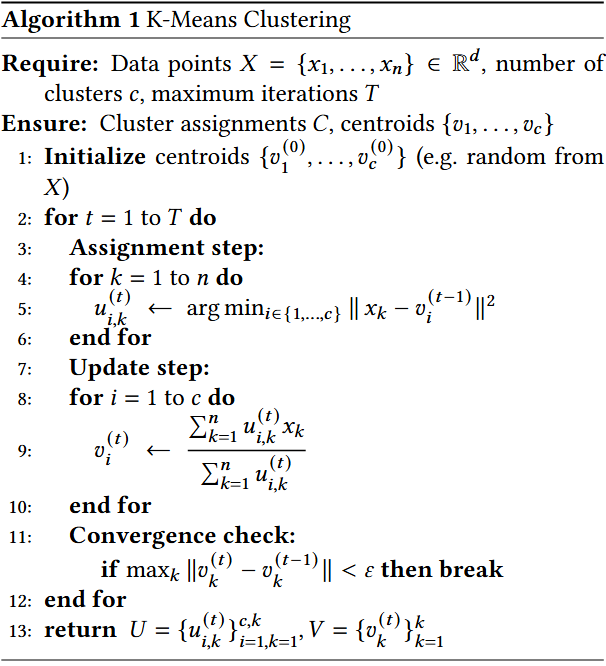
\includegraphics[width=\linewidth]{Figures/K-means_clustering.png}
%     \label{alg:kmeans}
% \end{figure}

\begin{algorithm}[ht]
\caption{K‐Means Clustering}
\label{alg:kmeans}
\begin{algorithmic}[1]
\REQUIRE Data points $X = \{x_1, \ldots, x_n\}\in\mathbb{R}^d$, number of clusters $c$, maximum iterations $T$
\ENSURE Cluster assignments $C$, centroids $\{v_1,\dots,v_c\}$
\STATE \textbf{Initialize} centroids $\{v_1^{(0)},\dots,v_c^{(0)}\}$ (e.g.\ random from $X$)
\FOR{$t = 1$ to $T$}
  \STATE \textbf{Assignment step:}
  \FOR{$k = 1$ to $n$}
    \STATE $u_{i,k}^{(t)} \;\leftarrow\; \arg\min_{i\in\{1,\dots,c\}}\|\,x_k - v_i^{(t-1)}\|^2$
  \ENDFOR
  \STATE \textbf{Update step:}
  \FOR{$i = 1$ to $c$}
    \STATE $\displaystyle v_i^{(t)} 
      \;\leftarrow\; 
      \frac{\sum_{k=1}^nu_{i,k}^{(t)}x_k}{\sum_{k=1}^nu_{i,k}^{(t)}}$
  \ENDFOR
  \STATE \textbf{Convergence check:} \\
    \hspace*{1em} \textbf{if} $\max_k \|v_k^{(t)} - v_k^{(t-1)}\| < \varepsilon$ \textbf{then break}
\ENDFOR
\RETURN $U = \{u_{i,k}^{(t)}\}_{i=1,k=1}^{c,k} ,V =\{v_k^{(t)}\}_{k=1}^k$
\end{algorithmic}
\end{algorithm}
% \ref{alg:kmeans}
One way of looking at this algorithm is following the traditional "guess and check" approach. After one round of centroid selection, entities are assigned to each centroid. Then the centroids are selected to minimize distance between the entities in a group and gradually that reach positions where they converge. 

\begin{figure}[!htpb]
    \centering
    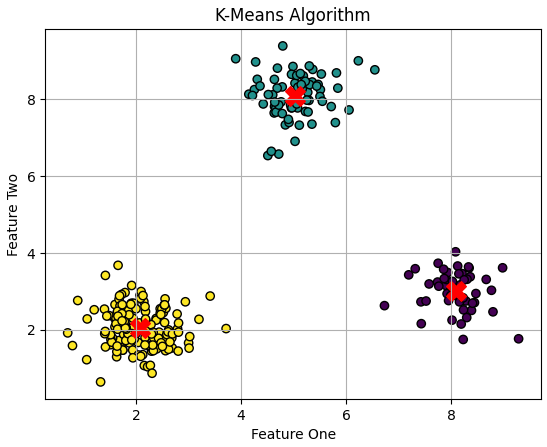
\includegraphics[width=\linewidth]{Figures/K-Means.png}
    \caption{Example of K-Means clustering on three distinct groups.}
    \label{fig:kmeans}
\end{figure}




\subsection{DC Algorithms}
%Breif review of DC functions, sufficient conditions, 
Difference of Convex Programming describes the Optimization Problem

\begin{equation}
    min \quad f(x) := g(x) - h(x), \quad \text{subject to } x \in R^d
    \label{dc function}
\end{equation}

\noindent where $g,h : R^d \;\rightarrow\; (-\infty,\infty] $ are convex. First introduced in \cite{tao_algorithms_1986} and expanded in many prolific works such has \cite{tao_convex_1997}, the resulting methods for solving these problems (know as DC algorithms(DCA)) have had use in many applications in machine learning and data science. While it it outside the scope of this work to provide a complete review of DCA, there are the following conditions. 
\begin{theorem}[Necessary condition for DCA]
 Suppose that $\bar{x}$ is a local minimizer of $f$ in \ref{dc function} then 
 \begin{equation}
 \partial h(\bar{x}) \subset \partial g(\bar{x})
\end{equation}

\label{thm:Necessary1}
\end{theorem}
\begin{theorem}[Sufficient condition for DCA]
 Suppose that there exists a neighborhood $\mathcal{N}$ of $\bar{x}$ such that 

\begin{equation}
    \varnothing \neq \partial h(x) \subset \partial g(\bar{x})
\quad\forall\,x\in \mathcal{N}.
\label{eq:suff1}
\end{equation}

\label{thm:Necessary1}
\end{theorem}

% One way of looking at this algorithm is following the traditional "guess and check" approach. After one round of centroid selection, entities are assigned to each centroid. Then the centroids are selected to minimize distance between the entities in a group and gradually that reach positions where they converge. 
% Finally, one addition from \cit{an_minimum_2009}.


% \begin{lemma}

% \cite{an_minimum_2009} Let $K$ be a nonempty bounded polyhedral convex set, $f$ be a DC function on $K$, and $p$ be a nonnegative concave function on $K$. Then there exists $t_0 \ge 0$ such that for all $t > 0$ the following problems have the same optimal value and the same solution set:
% \begin{align}
% \nonumber \quad(P) \quad \alpha = inf\{f(x):x\in K, p(x)\le 0  \} 
% \\
% \nonumber \quad \quad \quad (P_t) \quad \alpha (t) = inf\{f(x) +tp(x):x\in K, p(x)\le 0  \} 
% \end{align}
% \end{lemma}
\noindent The proofs and basic implementation of DCA for these are already covered in other works \cite{tao_convex_1997}. 
%Extensions beyond current classwork

\subsection{DCA for MSSC}
The works adapting DCA to MSSC include \cite{Ordin_heuristic_2015},\cite{artacho_boosted_nodate}, and many others outside the scope of this report. These are specifically related to rewriting equation \ref{eq:my_equatio}, as a difference of convex functions. \cite{an_minimum_2009} gives one natural adaptation. Note first that $u_{i,k} = u_{i,k}^2 \text{ as } u_{i,k} \in \{0,1\}$. 

Using the equation $f_1^2+ f_2^2 = (f_1+f_2)^2-2f_1f_2$ equation \ref{eq:my_equatio} can be rewritten as 
\[ f(U,V) = \sum_{k=1}^{n}\sum_{i=1}^{c}u_{i,k}^2 \|x_k - v_i\|^2 =\]
\[\frac{1}{2}\sum_{k=1}^{n}\sum_{i=1}^{c}(u_{i,k}^2 +\|x_k - v_i\|^2)^2-\frac{1}{2}(u_{i,k}^4+\|x_k - v_i\|^4).\]
Thus, \

\begin{equation}
    f(U,V):=G_1(U,V)-H_1(U,V)
\end{equation} 
where
\begin{equation}
G_1(U,V) = \frac{1}{2}\sum_{k=1}^{n}\sum_{i=1}^{c}(u_{i,k}^2 +\|x_k - v_i\|^2)^2
\end{equation} 
and
\begin{equation}
H_1(U,V)=\frac{1}{2}\sum_{k=1}^{n}\sum_{i=1}^{c}(u_{i,k}^4+\|x_k - v_i\|^4).
\end{equation} 

Note that each is the sum of convex functions and therefore also convex. This shows that $f(U,V)$ is a DC function. While the work \cite{an_minimum_2009} provides further information on how to adapt for implementation it comments, "this DC decomposition is not interesting because it requires an iterative algorithm for solving a convex program at each iteration."
\section{Methods}
In this section a reformation of DCA for MSSC is reviewed. It's main contribution is its convex subproblem is already known, reducing the total computation time. Additionally, some remarks about initialization processes for initial centroid selection are covered. 

\subsection{DCA Reformation}
In \cite{an_minimum_2009} an alternative formulation of DCA for MSSC is provided that solves the issues of having to resolve a convex subproblem at each step. In that work, equation \ref{dc function} is rewritten as
\begin{equation}
\min
\Bigl\{
\chi_{\Delta \times C}(U,V)
\;+\;
\frac{\rho}{2}\,\bigl\lVert (U,V)\bigr\rVert^2
\; \\
-\;
H_{2}(U,V)
:(U,V)\in \mathbb{R}^{c\times n}\times \mathbb{R}^{c\times d}\bigl\}.
\label{eq:dca18}
\end{equation}
where 
\begin{equation}
    H_2(U,V):=\frac{\rho}{2}\|(U,V)\|^2 -f(U.V),\quad G_2(U,V):=\frac{\rho}{2}\|(U,V)\|^2
\end{equation}



This first requires computation of the convex subprogram 
\begin{equation}
\min
\left\{
\frac{\rho}{2}\,\bigl\lVert (U,V)\bigr\rVert^2
\;-\,\bigl\langle (U,V),\,(Y^l,\,Z^l)\bigr\rangle:{(U,V)\in \Delta \times C}
\right\}.
\end{equation}
where
% \begin{equation}
%      %H_2=\bigr\langle\bigr\langle (V,U),(Y^l,Z^l
% \end{equation}
\begin{equation}
    \rho \ge \alpha^2+n+n \sqrt{[\frac{1}{n}\alpha^2+1]^2+\frac{16}{n}\alpha^2}\big]
\end{equation}
and 
\begin{equation}
    Y^l =\bigr(\bigr(\rho u^2_{i,k}-2 u^2_{i,k}\big)\|x_k-V^l_k\|^2+2tu^l_{i,k}-t\big)_{i=1,...c}^{k=1,...n}
    \label{Y}
\end{equation}
\begin{equation}
    Z^l=\bigr(\rho V_i^l-2\sum_{k-=1}^{n}(V^l_i-x_k)(u^2_{i,k})\bigr)_{i=1,...c}
    \label{Z}
\end{equation}
The solution is conveniently \cite{an_minimum_2009} provided as 
\begin{equation}
    (U^{l+1})^k= Proj_{\Delta k}\bigr((Y^l)^k) \text{ for } k=1,...n,
    \label{projectk}
\end{equation}
    
\begin{equation}
(V^{l+1})^k= Proj_{R_i}\bigr(\frac{1}{\rho}(Z^l)_i) \text {  for  } i=1,...c. 
\label{projectR}
\end{equation}
$\quad =\quad \bigg\{\frac{(Z^l)_i}{\rho} \text{ if } \|(Z^l)_i\| \le \rho r, \text{else }\frac{(Z^l)_ir}{ \|(Z^l)_i\|}, (i=1,...,c) $
\\

\noindent Essentially, equation \ref{projectk} is saying that the projection of $Y^k$ onto a simplex gives us the label assignment for the entities. While \ref{projectR} is projecting the results back into the outside edge of the ball containing all realistic possibilities. This is a significant result in terms of computation time for DCA as the convex subproblem that could potential take an unknown number of iterations is removed. This is perhaps the most interesting portion of this formulation. Together, the following DCA for the MSSC can be formulated in alg. \ref{alg:DCA}. 
\begin{algorithm}[ht]
\caption{DCA for MSSC}
\label{alg:DCA}
\begin{algorithmic}[1]
\REQUIRE Data points $X = \{x_1, \ldots, x_n\}\in\mathbb{R}^d$, number of clusters $c$, maximum iterations $L$, convergence threshold $\epsilon$
\ENSURE Cluster assignments $C$, centroids $\{v_1,\dots,v_c\}$
\STATE \textbf{Initialize} centroids $\{v_1^{(0)},\dots,v_c^{(0)}\}$ (e.g.\ random from $X$)
\textbf{Assign}  $X$ labels and store them in $U$ 
\FOR{$l = 1$ to $L$}
  \STATE \textbf{Compute subgradients} 
  \STATE $Y^l$ and $Z^l$ using equations \ref{Z} and \ref{Y}
  
  
  
  \STATE \textbf{Define set} 
  \STATE $U^l$ and $V^l$ $U^{l+1}$ and $V^{l+1}$ using equations \ref{projectR} and \ref{projectk} 
    \hspace*{1em} \textbf{if} $\max_k \|v_k^{(t)} - v_k^{(t-1)}\| < \varepsilon$ \textbf{then break}
\ENDFOR
\RETURN $U = \{u_{i,k}^{(t)}\}_{i=1,k=1}^{c,k} ,V =\{v_k^{(t)}\}_{k=1}^k$
\end{algorithmic}
\end{algorithm}

\subsection{Centroid initialization}
Initialization of optimization problems is always a prime issue. There are many works specifically looking at initialization procedures. For brevity, two basic initializations for an MSSC problem are going to be discussed here.
The first is random initialization within the solution space. In the case of MSSC, this involves calculating the min $\alpha_i$ and max $\beta_i$ for each dimension in $\mathbb{R}^d$. From here, the initial $c$ centroids can be guessed randomly within the space.

Other options take a heuristic approach. Instead, $c$ centroids are picked randomly from entities $X$. This can be further compounded by requiring a minimum distance $d$ to separate the centroids. A comparison of these two approaches will be covered in the results section.


% \begin{figure}[!htpb]
%     \centering
%     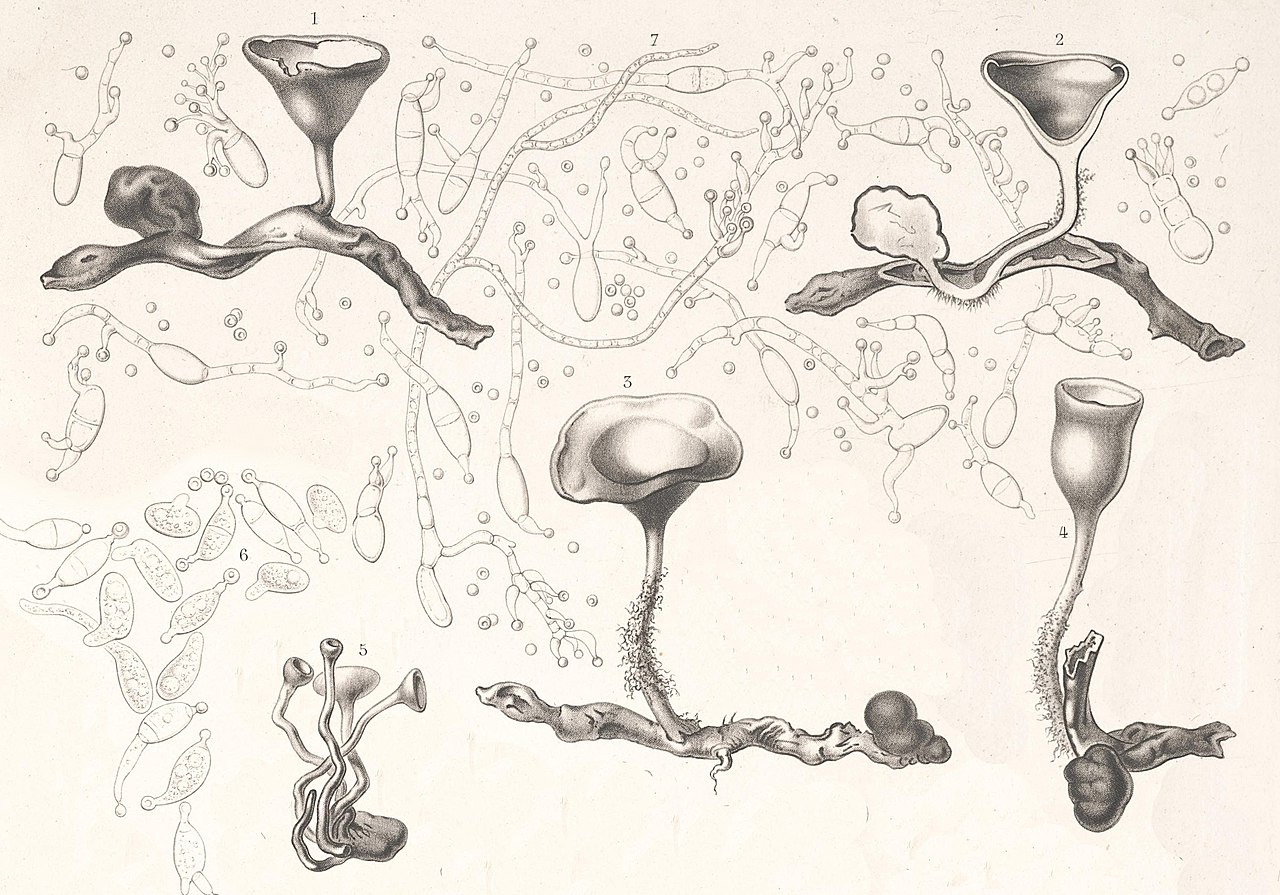
\includegraphics[width=\linewidth]{Figures/PezizaTuberosa.jpg}
%     \caption{Illustration of the fungus Dumontinia tuberosa by physician, mycologist, and illustrator Charles Tulasne (1816–1884) in the book Selecta Fungorum Carpologia (1861–65). (Name of the original work: Peziza tuberosa parasite on Anemone nemorosa).}
%     \label{fig:tcanther}
% \end{figure}

% \subsection{DCA for MSSC}
%example derivation of DC functions from MSSC. reference a few other versions. Point is to show that there are many DCA adaptations of MSSC 

% \subsubsection{Implented version}
%note sufficient versions, proof for rho, reference to T -- will not discuss much other than reference original material 

% \blindtext
% Results
\section{Experiments}
The following experiments were constructed to compare the K-means algorithm \ref{alg:kmeans} and the discussed DCA \ref{alg:DCA}. Experiment one tests the ability of each clustering algorithm to cluster in $\mathbb{R}^2$. Experiment two used the  1984 Congressional House-Votes  (VOTES) dataset \cite{noauthor_cluster_nodate}. In each case, the number of correctly grouped entities of the total number are reported.
\begin{@twocolumntrue}
\begin{table*}[ht!]
    \centering
    \caption{Experimental results for comparing the two clustering algorithms and initialization strategies. Results shown are for the average of $200$ cycles. Each the  initialization type $INIT$ number of elements $n$, the dimension in $\mathbb{R}^d$ and the number of clusters $c$ }
    \begin{tabular}{lllllllllll}
    \hline
        Experimental Results & ~ & ~ & ~ & ~ & K-Means & ~ & ~ & DCA & ~ &   \\ \hline
        Dataset & $n$ & $c$ & $d$ & $INIT$ & Accuracy & Time(s) & Iterations & Accuracy & Time(s) & Iterations  \\ 
        VOTE & 435 & 2 & 17 & Random & \ 87.23 & \ 4.11E-04 & \ 4.05 & 76.27 & 0.5978 & 229.41  \\ 
        VOTE & 435 & 2 & 17 & Heuristic & \ 87.70 & \ 1.66E-03 & \ 4.19 & 84.56 & 0.5250 & 201.21  \\ 
        2D  & 200 & 2 & 2 & Random & \ 77.14 & \ 4.74E-04 & \  5.06 & 71.12 & 0.3794 & 318.53  \\ 
        2D & 200 & 2 & 2 & Heuristic & \ 77.11 & \ 5.69E-04 & \ 5.79 & 73.9 & 0.3116 & 260.89  \\ \hline
    \end{tabular}
    \label{tab:exresults}
\end{table*}
\end{@twocolumntrue}
\subsection{Clustering in $\mathbb{R}^2$}
For the following experiment, 200 points were normally distributed about 2 randomly chosen centroids in a box $[-5,5]$. The number of points in each were randomly selected between $[50-150]$ at each iterations. 

\subsection{Party assignment}
The VOTES dataset consist of 435 data points with representative voting results on 17 actions and two possible political parties. This is formulated as each data point being a size 17 array with $1$, $-1$, and $0$ representing voting yay, nay, or unassigned.  



% \newpage


%This section introduces the 2-d triple cluster and the Voting predictions
% do experiments with initialization 



% \begin{table}[!htpb]
%     \caption{Clustering Algorithm Comparison.
% 	\textbf{R$_{max}$}: the performance in GFlops for the largest problem run on a machine; \textbf{N$_{max}$}: the size of the largest problem run on a machine; \textbf{N$_{1/2}$}: the size where half the \textbf{R$_{max}$} execution rate is achieved; \textbf{R$_{peak}$}: the theoretical peak performance in GFlops.}
%     \label{tab:table-01}
%     \centering
%     \begin{tabularx}{\linewidth}{rccccccccccc}
%         \toprule
%         \textbf{Linpack	Benchmark}& Proc. & \textbf{R$_{max}$} & \textbf{N$_{max}$} & \textbf{R$_{peak}$} \\ 
%         (Dataset) & or Cores	& $N$ & $C$ & $D$ & $init$\\ [0.25ex] 
%         \midrule
%         Thinking Machine CM-5 & 32 & 1,900 & 9216 & 4& \\
%         Pentium 4 3.0 GHz & 1 & 4,730 & 7600 & 6& \\
 
%         & & & & 14,6 \scriptsize{(64b)} \\
%         Thinking Machine SD-3 & 36 & 1,120 & 6728 & 3 \\
%         \bottomrule
%     \end{tabularx}
% \end{table}

% Please add the following required packages to your document preamble:
% \usepackage[table,xcdraw]{xcolor}
% Beamer presentation requires \usepackage{colortbl} instead of \usepackage[table,xcdraw]{xcolor}

% Discussion
\section{Discussion}

In table \ref{tab:exresults} the averages of 200 cycles with random seeds 0-199 are shown and a number of interesting results can be gleamed. The first is that it would appear that in both cases a heuristic based initialization improved the accuracy and time to completing of each of DCA on each of the test datasets. I believe this has to do with preventing ill-conditioned starting centroids such as have two place too close to each other and/or away from the rest of the entities. The second is that it would appear my implementation of the DCA from \cite{an_minimum_2009} appears to contain some mistake as my results do not agree with \cite{an_minimum_2009} on the same dataset VOTE. 
% Conclusion
\section{Conclusion}
This paper provide a brief introduce to the MSSC problem. It gave one formulation for thinking about the minimization problem as well as some algorithms. Overall, the results showed a benefit to using heuristic style initialization. The comparison between DCA and K-Means did not show an advantage to DCA, however this may be do to some computational mistake.

% \section*{Acknowledgements}
% This research received support during the XXX course, instructed by Professor XXX, PhD at the School of XXX, XXX.
\bibliographystyle{ieeetr}
\bibliography{Bibliography/Bibliography}
% \printbibliography

\end{document}
